\chapter{Ranking Biologically-Interesting SNPs in Incipient Species of Malaria Vectors using Random Forests}

\section{Abstract}
  Half of the world's population are at risk for malaria infection through vectors such as the mosquitoes \emph{Anopheles gambiae} and \emph{Anopheles coluzzii}.  Having recently diverged, the two species differ in feeding and mating habits as well as insecticide resistence but cannot be differentiated visually. Identifying genetic differences between the two species is key to understanding the biological differences and designing effective population-control efforts.
  Random Forests have been used in bioinformatics literature to identify subsets of genetic markers which describe phenotypic differences in studies as diverse as cancer and diabetes. 
  We use numerical experiments to illustrate the susceptibility of Random Forests to multiple sources of bias if not used with care, which affect variable importance score accuracy.
  We describe solutions to correct for bias and demonstrate that Random Forests can identify biologically-meaningful biallelic SNPs in insect vectors.

\section{Introduction}
The accumulation of genetic differences within separate populations may result in new species. Genetic differences between long-separated species often have macroscopic genomic differences such as re-ordered genes that are relatively easy to detect. During the early stages of speciation, however, genetic differences are often subtle, occurring in the form of differences in allele frequencies or combinations thereof. For example, the apple maggot \emph{Rhagoletis pomonella} separated from \emph{Rhagoletis zepheria} no more than two centuries ago, but allele frequencies likely changed rapidly \cite{Egan2015}.  Another classic example of recent speciation are the malaria vectors \emph{An. gambiae} and \emph{An. coluzzii} that were difficult to distingish genetically even after whole genome sequencing \cite{Lawniczak2010}. Tools and methods for identifying identifying genetic differences are valuable to efforts aiming to molecularly characterize such closely related species and ultimately understand underlying causes of speciation in these model systems.

Genetic differentiation of insects, however, faces several challenges. Although the genome sizes can be relatively small compared to human, collecting and sequencing enough samples is costly for these communities.  Further, many of these species have very little linkage disequilibrium (LD), for which single nucletide polymorphisms (SNPs) tend to be the primary feature (as opposed to larger haplotype blocks in species like human). Combined, currently available data sets tend to be ``wide'' with many features and few samples \cite{Lawniczak2010, Egan2015, Fontaine2015}.

Given the lack of LD, the typical method as applied to insect population genomics involve calculating multiple univariate statistics such as $F_{ST}$, nucleotide diversity ($\pi$), and Tajima's $D$ \cite{Fontaine2015}. Relatively diverged regions are isolated by atypical values, usually visualized across the genome \cite{Egan2015, Fontaine2015}. Due to the relatively small amount of information per SNP, a common strategy is to look at genome intervals (windows) in an attempt to amplify signal. Window-based analysis is able to find interactions between nearby SNPs but not larger interacting regions, especially in the absence of a previously competed reference genome \cite{Egan2015}.

Random Forests (RFs) offer an attractive alternative to more traditional techniques \cite{Breiman1999}. RFs are a versatile machine learning method that can be used for classification (supervised learning), variable selection, regression, and clustering (unsupervised learning).  RFs are able to utilize heterogenous features types such as real numbers or integers, categories, and ordinals. RFs also tend to perform well on data sets with numerous unlinked features such as genome-based SNPs with little LD \cite{Meng2009}.

RFs have started to see adoption across a range of problems in computational biology.  D\'{\i}az-Uriarte, et al. applied RFs to gene selection and classification from microarray data, finding that RFs perform in the case of a large number of noisy features \cite{Diaz-Uriarte2006}. Jiang, et al. successfully applied RFs to the classification of microRNA precursors \cite{Jiang2007}. Chen, et al. used RFs to predict protein-protein interactions \cite{Chen2005}. Kandaaswamy, et al. used RFs to identify anti-freeze proteins from sequence-derived features. RF clustering has been used by Shi, et al. to classify tumors from microarray data \cite{Shi2005}. Lin, et al. and Wu, et al. used RFs to identify DNA-binding proteins \cite{Lin2011}. Jiang, et al. applied RFs to predict SNP interactions associated with Age-related Macular Degeneration in a genome-wide associated study \cite{Jiang2009}. Lunetta, et al. also applied RFs to predicting SNP interactions in a large-scale association study \cite{Lunetta2004}.  Liu, et al. applied RFs to identifying protein-RNA binding sites \cite{Liu2010}. Moore, et al. reviewed computational challenges in genome-wide association studies, arguing for Random Forests as one solution \cite{Moore2010}.

Researchers have begun to identify challenges associated with using RFs for bioinformatics problems and extensions to RF methods. Strobl, et al. identified issues with bias in RF variable importance scores associated with categorical variables and bootstrap resampling of samples during training and proposed a new method called ``cforest'' \cite{Strobl2007}. Nicodemus, et al. analyzed bias present in RF permutation-based variable importance measures \cite{Nicodemus2010}. To overcome identified issues, Strobl, et al. proposed the Conditional Random Forest method \cite{Strobl2008}. Altmann, et al. proposed using permutation importance as variable importance measure that avoids bias present in the more traditional Gini importance measure \cite{Altmann2010}. Calle, et al. compared two common variable importance measures, mean decrease accuracy and mean decrease Gini, finding that mean decrease Gini is more stable in the face of small perturbations \cite{Calle2011}. Amaratunga, et al. proposed using weights so that features are not sampled uniformally in splits, calling the method Enriched Random Forests \cite{Amaratunga2008}.

We consider the problem of apply RFs to challenging whole-genome studies of early speciation of insects. We use simulated data sets to demonstrate that RFs are susceptible to multiple sources of bias, in line with previous work by Strobl, et al \cite{Strobl2007, Strobl2008, Nicodemus2010} and Altmann, et al. \cite{Altmann2010}. Unlike the previous work, we describe a solutions that can be used with common ``out-of-the-box'' implementations of decision trees. We apply our solutions to ranking SNPs, which we validate by identifying SNPs associated with incipient speciation of insect vectors.  Our workflow is implemented in and available through an open-source software package written in Python using the Numpy and scikit-learn libraries.


\section{Methods and Implementation}


\subsection{Variable Transformation}
The first stage is conversion of input SNP data into a data representation suitable for Random Forest construction.  Aranyani expects a VCF file containing $M$ phased SNP variants for $N$ individuals and a file mapping the individuals' IDs to populations.  Aranyani converts the input VCF file into a feature matrix consisting of Boolean-valued columns, known as ``one-hot encoding.'' For each SNP, a Boolean-valued (represented as 0s and 1s) column is created for each nucleotide value (A, T, C, G) present in the individuals.  Unknown nucleotides (X) are represented by 0 (false) values in all of the columns.  The four columns for each haploid are mutually-exclusive -- only one column can have a 1 (true) value.  One-hot encoding is used to prevent bias in the machine learning models due to varying sizes of the categorical variables.

Table~\ref{tab:snp-examples} contains examples of SNP values for three individuals with the resulting feature matrix in Table~\ref{tab:features-example}.  The SNPs are labeled by triplets of chromosome, position, and haploid.  The first SNP (1, 1, 1) is represented by two columns ((1, 1, 1, A) and (1, 1, 1, T)) in the feature matrix since the individuals have two nucleotides (A and T) between them. Individuals 1 and 3 have 1s in column 1 (1, 1, 1, A) and 0s in column 2 (1, 1, 1, T) of the features matrix since their SNP values are A, while individual 2 has a 0 in column 2 (1, 1, 1, A) and a 1 in column 2 (1, 1, 1, T).

Note that unknown nucleotides (X) do not receive their own columns.  In cases where individuals have an unknown nucleotide, 0s are placed in all columns for that SNP.  For example, individual 3 has 0s in columns 4 (1, 10, 1, C), 5 (1, 10, 1, G), and 6 (1, 10, 2, A) since the nucleotides are unknown for those SNPs.

\begin{table}[h!]
  \begin{center}
    \begin{tabular}{ c c c c c }
      \hline
      \textbf{Individual} & \textbf{(1, 1, 1)} & \textbf{(1, 1, 2)} & \textbf{(1, 10, 1)} & \textbf{(1, 10, 2)} \\ \hline
      1 & A & T & C & X \\
      2 & T & T & G & A \\
      3 & A & T & X & X \\
    \end{tabular}
  \end{center}
  \caption{Examples of SNP values for three individuals.  The SNPs are labeled by triplets of (chromosome, position, haploid).}
  \label{tab:snp-examples}
\end{table}

\begin{table}[h!]
  \begin{center}
    \begin{tabular}{ c c c c c c c}
      \hline
      \textbf{Individual} & \textbf{(1, 1, 1, A)} & \textbf{(1, 1, 1, T)} &\textbf{(1, 1, 2, T)} & \textbf{(1, 10, 1, C)} & \textbf{(1, 10, 1, G)} &\textbf{(1, 10, 2, A)} \\ \hline
      1 & 1 & 0 & 1 & 1 & 0 & 0 \\
      2 & 0 & 1 & 1 & 0 & 1 & 1 \\
      3 & 1 & 0 & 1 & 0 & 0 & 0 \\
    \end{tabular}
  \end{center}
  \caption{Feature matrix for three individuals in Table~\ref{tab:snp-examples}.  The features are labeled by quartets of (chromosome, position, haploid, nucleotide value).}
  \label{tab:features-example}
\end{table}

After populating the feature matrix, the columns that have same value either because there are no SNPs or all individuals have the same genotype are removed.  Filtering prevents errors in the machine learning models, reduces memory and disk usage, and improves run times.  We use two criteria for filtering columns. SNPs where individuals all have the same value result in a single feature column with all 1s.  Such a SNP offers no information for distinguishing between individuals and are filterd out.  For an example, see SNP column 2 (1, 1, 2) in Table~\ref{tab:snp-examples} represented by feature column 3 (1, 1, 2, T) in Table~\ref{tab:features-example}.

Likewise, SNPs with only one known nucleotide value are also filtered out. The feature columns may contain both 1s and 0s (in the case of unknown nucleotides).  For example, see SNP column 4 (1, 10, 2) in Table~\ref{tab:snp-examples} represented by feature column 6 (1, 10, 2, A) in Table~\ref{tab:features-example}.  Although the values would distinguish between individuals, we would be classifying individuals based on unknown information -- we do not want the machine learning models to associate an unknown value (X) as different from a known value (T).  This could lead to errors in classifications since the unknown value might actually be one of the known values.

Table~\ref{tab:filtered-features-example} gives the result of filtering the feature matrix in Table~\ref{tab:features-example}. Columns 3 (1, 1, 2, T) and 6 (1, 10, 2, A) were removed since they match the first and second criteria, respectively.

\begin{table}[h!]
  \begin{center}
    \begin{tabular}{ c c c c c }
      \hline
      \textbf{Individual} & \textbf{(1, 1, 1, A)} & \textbf{(1, 1, 1, T)} & \textbf{(1, 10, 1, C)} & \textbf{(1, 10, 1, G)} \\ \hline
      1 & 1 & 0 & 1 & 0 \\
      2 & 0 & 1 & 0 & 1 \\
      3 & 1 & 0 & 0 & 0 \\
    \end{tabular}
  \end{center}
  \caption{Filtered feature matrix for three individuals in Table~\ref{tab:snp-examples}.  The features are labeled by quartets of (chromosome, position, haploid, nucleotide value).}
  \label{tab:filtered-features-example}
\end{table}

\subsection{Ranking SNPs}
SNPs are ranked by their ``variable (feature) importance'' scores computed from the decision trees in a Random Forest model.  A decision tree encodes how combinations of feature values uniquely identify one class (group) of individuals from another.  Decision trees are generated by choosing a feature and thresholding its values into two groups at every split in the tree.  The particular feature and threshold are chosen to maximize the sorting individuals by class according to an objective function such as the Gini impurity. Trees are grown until either a maximum depth is reached, a number of samples in a leaf node have reached a given minimum, or leaf nodes have homogenous values (all individuals are from the same class).

A Random Forest is an ensemble of decision trees with uses bagging of individuals and random subsampling of features.  For every decision tree in a Random Forest, the individuals are resampled (known as bootstrapping or bagging) from the original set of individuals and a randomly-chosen subset of features are chosen for training the tree. The addition of the two sampling procedures increases variation among the trees and enables exploring a wide range of feature combinations.

After training the random forest, we compute the SNP importance scores from the features' variable importance scores, calculated for each feature by averaging and scaling their objective function values.  Features used in nodes closer to the top of tree generally have higher variable importance scores.  Features' variable importance scores are averaged across all of the trees in the Random Forest.  The variable importance scores for each SNP are calculated by averaging the variable importance scores of the corresponding features.  For example, the variable importance score for the SNP of column 1 (1, 1, 1) in Table~\ref{tab:snp-examples} would be calculated as the average of the scores for features of columns 1 (1, 1, 1, A) and 2 (1, 1, 1, T) in Table~\ref{tab:filtered-features-example}.  SNPs with importance score of zero (i.e., SNPs that haven't been sampled by the Random Forests) are filtered out.  The remaining SNPs are ranked according to their importance scores.  SNPs with higher importance scores are higher in the rankings.

\textcolor{red}{Provide example of calculations}


\subsection{Effect of Tree Counts on SNP Importance Score Convergence}
Parameters for the Random Forests include the number of trees, the number of features to sample, the maximum depth, and the minimum number of individuals needed to split a node.  We use a minimum split size of two and set the maximum depth to a large number.  Since the number of individuals used in biological work is very small (tens of individuals), the trees tend to be quite small, utilizing only tens of features and with depths of $<$10.  We found that randomly sampling $\sqrt{n_{features}}$ leads to the fastest convergence (in terms of number of trees) of the SNP importance scores.  This leaves the number of trees as the only parameter that the user must set.  More trees leads to less variance in the SNP importance scores.

We provide an analysis approach to guide the user in determining the number of trees needed for the SNP importance scores to converge.  We sweep over the number of trees, training two Random Forest models for each parameter value.  SNPs' importance scores are computed from each model and ranked.  The top ranked SNPs from each model, for a set of thresholds provided by the user, are compared to identify the percentage of SNPs in common.  If the two models are converged, 100\% of the SNPs should be the same for any ranking threshold. The common percentage of SNPs for various thresholds as a function of the number of trees are reported in a plot (see Figure~\ref{fig:ranking-convergence-analysis}).  The user can use the plot as a guide for choosing the number of trees.

\subsection{Software Implementation}
Aranyani is implemented in Python using the Numpy, Scikit Learn, and Matplotlib libraries.  Aranyani has an extensive set of unit tests to prevent defects and make changes easier to make.  The Random Forests functionality is provided by Scikit Learn. Numpy memory-mapped arrays are used to support feature matrices larger than available RAM.   Aranyani is available under the Apache License v2 at \url{http://www.github.com/rnowling/aranyani}.

\textcolor{red}{extend when software is developed}

\section{Results}

\subsection{Bias from Encoding of Categorical Variables}
Analysis by Strobl, et al. \cite{Strobl2007} and Altmann, et al. \cite{Altmann2010} found that variable importance scores from Random Forests were biased towards categorical variables with more categories.  Genomic data primarily consists of categorical variables, making categorical variable bias an important issue.  We re-created Altmann, et. al.'s simulation studies to study the effect of encoding schemes on variable importance of categorical variables.  We randomly generated 100 datasets with 1000 samples and uninformative 31 categorical variables with 2-32 categories each.  The values of the categorical variables were sampled from an uniform distribution so that each category had an equal chance of being chosen and no correlation with the output labels. Random Forests with 100 trees were trained on each dataset and used to compute variable importance scores.

We evaluated two encoding schemes: integer encoding and one-hot encoding.  Under the integer encoding scheme, each of the 31 categorical variables was encoded as a column in the feature matrix with the categories represented as integers starting from 0.  In one-hot encoding, each category variable of $N$ categories is encoded as $N$ columns of 0's and 1's.  The columns are mutually exclusive such that only one of the columns can be ``hot,'' or have value of 1 for each sample.  The resulting feature matrix had 527 columns.  When computing the variable importance score for each one-hot encoded categorical variable, we averaged the variable importance scores from the columns associated with that variable.

In our simulation studies, we found that the bias observed by Altmann, et al. \cite{Altmann2010} may have been due to the encoding scheme used; we observed the bias reported by Altmann, et al. with integer encoding but not one-hot encoding. We would expect the variable importance scores to be equal across all of the variables since each variable is equally uninformative.  As the box plots in Figure~\ref{fig:integer} demonstrate, variables with more categories have higher variable importances with integer encoding.   When using one-hot encoding, however, the variable importances are uniform (see Figure~\ref{fig:one-hot}), regardless of the number of categories.  Our results suggest that the bias observed by Altmann, et al. may have been a result of the encoding scheme and can be corrected by using one-hot encoding.

% integer encoding used commonly in bioinformatics.  nucleic acids, amino acids, etc.

\subsection{Bias from Unknown Genotypes}
Due to sequencing and assembly challenges of the genomes of non-model organisms, SNPs for some samples may have unknown genotypes.  We generated synthetic data to analyze the effect of missing data on the variable importance scores.  We simulated 12 biallelic SNPs with possible values of A/A, A/T, and T/T.  Each SNP was encoded as two features, giving the number of As and Ts respectively.  For example, A/A becomes (2, 0), A/T becomes (1, 1), and T/T becomes (0, 2).  The SNPs are organized into four groups of three.  The first three SNPs are chosen from a uniform distribution and uncorrelated with the output labels.  The remaining three groups of SNPs have 100\%, 75\%, and 50\% probabilities, respectively, of being correlated with the output label. To simulate the effect of missing data, we zeroed out the features of the first, second, and third SNP in each group for 0, 10, and 20 randomly-chosen individuals.  We generated 100 datasets with 100 samples each and trained a RF with 100 trees on each dataset.  

The variable importance scores are plotted in Figure~\ref{fig:missing-data}.  The variable importance scores for features with no missing data are shown in Figure~\ref{fig:missing-data-none}, while the variable importance scores with the missing data are shown in Figure~\ref{fig:missing-data-missing}.  Each sequential pair of variables correspond to a SNP.  For example, variables 1 and 2 correspond to SNP 1. Variables 7-12 correspond to the SNPs with perfect correlation to the output label, 13-18 correspond to SNPs with 75\% correlation, and SNPs 19-24 correspond to the variables with 50\% correlation.

Figure~\ref{fig:missing-data-missing} demonstrates that removing data for 10 (or 10\%) and 20 (or 20\%) of the individuals leads to significant decreases in the variable importance scores.  Variables 7-8 have significantly higher variable importance scores than variables 9-10 and 11-12. In our control (Figure~\ref{fig:missing-data-none}), all of these variables have the same importance scores.

Unknown genotypes are a characteristic of the data set, not the underlying biology.  Penalizing SNPs with important biological function due to missing data for some individuals may not desirable. Imputation is a commonly-used approach in machine learning to overcome the problem of missing data.  The most popular approach is to filling in missing data with an average of the known values from individuals in the same class.  Since we're using discrete data, we chose to evaluate using the mode, or most common value, for imputation.  Simulations were carried in the same manner as for the missing data, but individuals' missing values were replaced with the most common value from individuals in the same class.  The resulting variable importance scores are shown in Figure~\ref{fig:missing-data-imputed}.  Imputing the data with the mode ``recovers'' the original variable importance scores, demonstrating that imputation can be used successfully to overcome bias due to missing data.

\subsection{Effect of Number of Variables and Correlated Variables on Variable Importance Scores} \label{sec:correlated}
The variable importance scores are calculated at two levels.  For each tree, the mean decrease in impurity is calculated for each feature used.  Features that are not used in a tree receive a mean decrease of 0 for that tree.  The variable importance scores are then calculated by taking the average of the mean decreases in impurity for each feature across all of the trees.

\[
VIM_f = \frac {1} {N_t} \sum_{t=1}^{N_t} \bar{\Delta}_{f, t}
\]

where $\bar{\Delta_{f, t}}$ is the mean decrease in impurity of feature $f$ for tree $t$ and $N_t$ is the total number of trees.

In the case where we have a large number of features but a small number of samples, only a small number of features will be used in each tree.  As a result, the feature importance scores will be down-weighted by a large number of 0's and vary with the number of trees used.

We used synthetic data set to evaluate the effect of the number of variables on feature importance scores.  We randomly generated data sets of 10 samples with 5, 10, and 25 uncorrelated binary variables.  The output labels were sampled uniformally from $\{0, 1\}$.  Variable importance scores were computed from Random Forests with 100 trees.  We ran 100 simulations.  The distributions of variable importance scores are plotted in Figure~\ref{fig:var-count}.  As the number of variables increased from 5 to 10 and 25, the variable importance score for each variable decrease.

Correlation between informative variables introduces another source of bias. We used simulations to evaluate the effect of variable correlation on variable importance scores. We randomly generated data sets of 10 samples with 25 binary variables.  The data sets had 1, 10, and 25 features with values correlated with the output label and each other. The output labels were sampled uniformally from $\{0, 1\}$. Variable importance scores were computed from one Random Forest with 100 trees per simulation.  We ran 100 simulations.

The distributions of variable importance scores and number of times each feature was used in a tree are plotted in Figure~\ref{fig:corr-1}.  As the number of correlated features increased, the variable importance scores of each feature decreased.  The number of times each feature was selected also decreased.  Since each tree only needed to selected a subset of the correlated features, the number of selected variables decreased, down-weighting the variable importance scores.

Our analysis suggest that the bias in variable importance scores for correlated variables are due to each variable being chosen less frequently as the number of variables increase.  For our use case, the number of informative features is large and the number of features used per tree is small.  As such, informative features are not chosen more often than they are chosen, causing their variable importance scores to be down-weighted by a large number of zeros (the default variable importance scores when a variable is not selected).

\textcolor{red}{are scores of correlated variables distinguishable from uncorrelated variables even with large numbers of variables?}

\subsection{Bias from Re-sampling} \label{sec:resampling}
Random Forests employ ``bootstrap aggregation,'' or bagging, to improve classification accuracy on classifiers which are unstable \cite{Breiman1996}.  Unstable classifiers like decision trees may generate models that differ greatly when small changes are made to the training set.  Bagging compensates by re-sampling the original training set for each tree trained, thus accounting for variations in possible data sets frequencies.  Bagging employs two steps: 1) bootstrap resampling of the original training set to create a new training set for each decision tree and 2) employing a majority-vote scheme for classification in which each decision tree gets one vote.

With small sample sizes such as 10 or 20 samples, individual samples are frequently excluded from re-sampled data sets.  Consider a variable with values that are split along class lines for all but one or two samples. Due to the high frequency with which the one or two samples with confounding values will be excluded from the re-sampled data sets, the variable will have a mean decrease impurity of 1 from some of the decision trees. 

For our use case, our goal is to obtain variable importance scores that are accurate relative to the genotypes present in the original population; classification accuracy is not our concern.  If we observe a genotype in one of the samples, we know that genotype is present in the original population. We don't want to exclude any of the observed genotypes, even if those genotypes have a very low frequency of occurrence in the original population.  As a consequence, bagging can cause the variable importance scores of variables with one or two samples with confounding values will be larger than expected, and thus, biased.

We propose ``constrained bagging'' in sampled copies are added to the original training set rather than replacing samples.  Each re-sampled training set contains the original training set plus zero or more additional samples.   With zero re-samples, there is no variance in the re-sampled training sets.  With a small number of the re-samples, the sample occurrences have a high probability of being skewed relative the frequencies of the original training set.  As the number of re-samples increases, the distribution of sample occurrences have a high probability of being equal to the frequencies fo the original training set.  As a result, the number of re-samples controls the variance in the sample occurrence counts, a property of multinomial models.

We evaluated the effects of bagging and contrained bagging on mean decreases in impurity using simulations.  We randomly generated data sets of ten samples with none binary variables. The data sets had two classes with five samples assigned to each.  Seven of the variables were uncorrelated -- values were chosen uniformally from $\{0, 1\}$. One of the variables was correlated with the output label.  And lastly, one of the variables was correlated with the output label for all but one sample, which had a value equal to the output label for the other class.  Distributions of mean decrease in impurities were calculated using 10,000 decision trees.

Figure~\ref{fig:bagging-bias} shows the distribution of mean decreases in impurity for a confounded variable with bagging and contrained bagging with 0, 10, 100, and 1000 additional re-samples.  With bagging, the mean decrease in impurity is calculated as 1 for 10\% of the decision trees, evidence of the situation we want to avoid.  With zero additional re-samples, the mean decrease in impurity is frequently in the range $[0.65, 0.70)$ but does not incorporate the possible variance in the frequencies of the genotypes in the underlying population.  By adding 10, 100, and 1000 re-samples, the sample frequencies are allowed to fluctuate to estimate possible frequency distributions that could be present in the underlying population.  With a smaller number of re-samples, the impurities vary significantly, while the impurity distribution begins to converge to that with no re-samples when using a large number of re-samples.

\subsection{Determining Number of Trees Needed for Stable Rankings}

\subsection{Software}
We combined one-hot encoding, genotype imputation, constrained bagging, and our methodology for determining the number of trees needed for stable ranking of SNPs to form a workflow for ranking SNPs.  We implemented our workflow in a Python software packaged called ``Asaph'' using the Numpy and scikit-learn libraries.  Asaph is available under the open-source Apache License v2 at \url{https://github.com/rnowling/asaph}.

To reduce run times and memory usage, we employed dictionary compression on the columns of the feature matrix. Duplicate variables are grouped and replaced with a single instance.  A mapping between the original variables and replacement variable is maintained.  We can set the variable importance score for each variable in a duplicated set equal to the score of the single remaining variable.

When applied to the SNPs of \emph{An. funestus}, dictionary compression reduced the number of features from 4,472,916 to 49,924, a reduction of 98.9\%.   This suggests that biological data sets may have a significant number of duplicated variables.  By reducing the number of variables to 1\% of the original size, run times were $\approx100 \times$ faster, reduced from hours to minutes.

\subsection{Application to \emph{An. gambiae} and \emph{An. coluzzii}}
We applied ``Asaph'' to analysis of SNPs from the malaria vectors \emph{An. gambiae} and \emph{An. coluzzii}, two incipient species of mosquitoes.

\begin{table}[h!]
  \begin{center}
    \begin{tabular}{ c c c p{8cm} }
      \hline
      \textbf{Chromosome} & \textbf{Position} & \textbf{Score} & \textbf{Notes} \\ \hline
      2L & 25396564 & 0.00032 &  \emph{resistance to dieldrin (Rdl)} gene associated with insecticide resistance (\textcolor{red}{Lawnziak et al, 2009})\\
      2L & 11568165 & 0.00032 &  \\
      2L & 21707904 & 0.00031 &  \\
      X  & 18853272 & 0.00122 &  \\
      X  & 19789366 & 0.00121 &  \\
      X  & 20141128 & 0.00121 & Intron 2-3 of Armadillo segment polarity protein (AGAP001043-RA) (\textcolor{red}{Neafsey et al, 2009})\\
      X  & 18927357 & 0.00119 & Intron 1-2 of cuticular protein (AGAP000986-RA) \\
      X  & 15271290 & 0.00118 &  \\
      X  & 14564483 & 0.00118 &  \\
      X  & 18441856 & 0.00117 & Intron 2-3 of nicotinic acetylcholine receptor subunit alpha 7 (AGAP000962-RA) (\textcolor{red}{Neafsey et al, 2009})\\
      X  & 19820035 & 0.00115 &  \\
      X  & 19513702 & 0.00112 & Intron 5-6 of notch gene homolog 1 (AGAP001015-RA) (\textcolor{red}{Neafsey et al, 2009})\\
    \end{tabular}
  \end{center}
  \caption{Fixed Differences from the top-ranked SNPs for 2L and X chromosomes of \emph{An. gambiae} vs \emph{An. coluzzii}.}
  \label{tab:filtered-features-example}
\end{table}

\subsection{Application to \emph{An. funestus}}
\emph{An. funestus} mosquitoes, along with \emph{An. gambiae}, are a major vector of malaria in Africa \textcolor{red}{cite}. Recent studies have shown that \emph{An. funestus} has two chromosomal forms, Folonzo and Kiribina.  We analyzed 1,874,475 SNPs from 10 samples, five of each chromosomal form, using our Asaph software.  We used dictionary compression and 1 million trees.

Variable importance scores of all of the SNPs, sorted by rankare shown in Figure~\ref{fig:funestus-all}.  We distinguish between the 7,156 SNPs (red) that trivially separate the two forms (the genotypes of each form are disjoint) and the rest, which we call ``confounding.''  We note that the Random Forests are unable to distinguish between trivial SNPs; any small differences in variable importance scores are a result of small differences in the number of times each SNP was sampled.  Trivial SNPs include fixed differences as well as SNPs in which one form may have two genotypes.  Methods like $F_{ST}$ downweight SNPs with variation within a population, allowing them to distinguish between fixed differences and other forms that trivial SNPs can take.

We observe several gaps in variable importances of groups of SNPs.  The trivial SNPs have variable importance scores $> 10^{-3}$.  A smaller block of 503 confounding SNPs has VIMs between $4\times 10^{-4}$ and $6\times 10^{-4}$.  A third, larger block of 26,078 SNPs have VIMs in the range of $3\times 10^{-4}$ and $1\times 10^{-4}$.  




Resistance to pyrethroid insecticides has been observed in \emph{An. funestus}, affecting population control efforts \textcolor{red}{cite}.   

\section{Discussion}

\section{Conclusion}

\section{Figures}

\pagebreak

\begin{figure}[H]
  \centering
  \begin{subfigure}[b]{0.45\textwidth}
    \includegraphics[width=\textwidth]{figures/random_forests/rf_bias_integer}
    \caption{Integer Encoded}
    \label{fig:integer}
  \end{subfigure}
  ~
  \begin{subfigure}[b]{0.45\textwidth}
    \includegraphics[width=\textwidth]{figures/random_forests/rf_bias_onehot}
    \caption{One-Hot Encoded}
    \label{fig:one-hot}
  \end{subfigure}
  \caption{Comparison of effect of encoding schemes for categorical variables on variable importance scores. The variables have randomly-chosen values with no correlation with output labels and 2-32 categories.}
  \label{fig:encoding-schemes}
\end{figure}

\begin{figure}[H]
  \centering
  \begin{subfigure}[b]{0.45\textwidth}
    \includegraphics[width=\textwidth]{figures/random_forests/rf_missing_data_none}
    \caption{No Missing Data}
    \label{fig:missing-data-none}
  \end{subfigure}
  ~
  \begin{subfigure}[b]{0.45\textwidth}
    \includegraphics[width=\textwidth]{figures/random_forests/rf_missing_data}
    \caption{Missing Data}
    \label{fig:missing-data-missing}
  \end{subfigure}
  ~
  \begin{subfigure}[b]{0.45\textwidth}
    \includegraphics[width=\textwidth]{figures/random_forests/rf_missing_data_imputed_mode}
    \caption{Missing Data Imputed with Mode}
    \label{fig:missing-data-imputed}
  \end{subfigure}
  \caption{Effect of missing data on variable importance scores.}
  \label{fig:missing-data}
\end{figure}

\begin{figure}[H]
  \centering
  \begin{subfigure}[b]{0.45\textwidth}
    \includegraphics[width=\textwidth]{figures/random_forests/rf_variable_count_bias_5.png}
    \caption{5 Uninformative Variables}
    \label{fig:var-count-5}
  \end{subfigure}
  ~
  \begin{subfigure}[b]{0.45\textwidth}
    \includegraphics[width=\textwidth]{figures/random_forests/rf_variable_count_bias_10.png}
    \caption{10 Uninformative Variables}
    \label{fig:var-count-10}
  \end{subfigure}
  ~
  \begin{subfigure}[b]{0.45\textwidth}
    \includegraphics[width=\textwidth]{figures/random_forests/rf_variable_count_bias_25.png}
    \caption{25 Uninformative Variables}
    \label{fig:var-count-25}
  \end{subfigure}
  \caption{Distributions of variable importance scores with 5, 10, and 25 uninformative variables.}
  \label{fig:var-count}
\end{figure}

\begin{figure}[H]
  \centering
  \begin{subfigure}[b]{0.45\textwidth}
    \includegraphics[width=\textwidth]{figures/random_forests/rf_correlated_1_0_1.png}
    \caption{1 Correlated Variable}
    \label{fig:corr-1-1}
  \end{subfigure}
  ~
  \begin{subfigure}[b]{0.45\textwidth}
    \includegraphics[width=\textwidth]{figures/random_forests/rf_correlated_1_0_1_feature_counts.png}
    \caption{1 Correlated Variable}
    \label{fig:corr-1-1-counts}
  \end{subfigure}
  ~
  \begin{subfigure}[b]{0.45\textwidth}
    \includegraphics[width=\textwidth]{figures/random_forests/rf_correlated_1_0_10.png}
    \caption{10 Correlated Variables}
    \label{fig:corr-1-10}
  \end{subfigure}
  ~
  \begin{subfigure}[b]{0.45\textwidth}
    \includegraphics[width=\textwidth]{figures/random_forests/rf_correlated_1_0_10_feature_counts.png}
    \caption{10 Correlated Variables}
    \label{fig:corr-1-10-counts}
  \end{subfigure}
  ~
  \begin{subfigure}[b]{0.45\textwidth}
    \includegraphics[width=\textwidth]{figures/random_forests/rf_correlated_1_0_25.png}
    \caption{25 Correlated Variables}
    \label{fig:corr-1-25}
  \end{subfigure}
  ~
  \begin{subfigure}[b]{0.45\textwidth}
    \includegraphics[width=\textwidth]{figures/random_forests/rf_correlated_1_0_25_feature_counts.png}
    \caption{25 Correlated Variables}
    \label{fig:corr-1-25-counts}
  \end{subfigure}
  ~
  \caption{Analysis of variables from generated data sets with 1, 10, and 25 out of 25 variables perfectly correlated with the output label. The left-hand side figures are distributions of variable importance scores. Right-hand side figures are number of trees using each variable.}
  \label{fig:corr-1}
\end{figure}

\begin{figure}[H]
  \centering
  \begin{subfigure}[b]{0.45\textwidth}
    \includegraphics[width=\textwidth]{figures/random_forests/bagging_bias_bagging_hist.png}
    \caption{Bagging}
    \label{fig:bagging-bias-bagging}
  \end{subfigure}
  ~
  \begin{subfigure}[b]{0.45\textwidth}
    \includegraphics[width=\textwidth]{figures/random_forests/bagging_bias_no_bagging_hist.png}
    \caption{Constrained Bagging, 0 Resamples}
    \label{fig:bagging-bias-constrained-0}
  \end{subfigure}
  ~
  \begin{subfigure}[b]{0.45\textwidth}
    \includegraphics[width=\textwidth]{figures/random_forests/bagging_bias_constrained_bagging_hist_10.png}
    \caption{Constrained Bagging, 10 Resamples}
    \label{fig:bagging-bias-constrained-10}
  \end{subfigure}
  ~
  \begin{subfigure}[b]{0.45\textwidth}
    \includegraphics[width=\textwidth]{figures/random_forests/bagging_bias_constrained_bagging_hist_100.png}
    \caption{Constrained Bagging, 100 Resamples}
    \label{fig:bagging-bias-constrained-100}
  \end{subfigure}
  ~
  \begin{subfigure}[b]{0.45\textwidth}
    \includegraphics[width=\textwidth]{figures/random_forests/bagging_bias_constrained_bagging_hist_1000.png}
    \caption{Constrained Bagging, 1000 Resamples}
    \label{fig:bagging-bias-constrained-1000}
  \end{subfigure}
  ~
  \caption{Distributions of mean decreases in impurity when using bagging and constrained bagging with 0, 10, 100, and 1000 additional re-sampled instances.}
  \label{fig:bagging-bias}
\end{figure}

\begin{figure}[H]
  \centering
  \begin{subfigure}[b]{0.45\textwidth}
    \includegraphics[width=\textwidth]{figures/random_forests/snp_counts}
    \caption{Sampled SNP Counts}
    \label{fig:ranking-counts}
  \end{subfigure}
  ~
  \begin{subfigure}[b]{0.45\textwidth}
    \includegraphics[width=\textwidth]{figures/random_forests/common_snps}
    \caption{Common SNPs by Rank}
    \label{fig:ranking-common}
  \end{subfigure}
  \caption{Analysis of sampled SNPs and common SNPs by rank.}
  \label{fig:ranking}
\end{figure}

\begin{figure}[H]
  \centering
  \begin{subfigure}[b]{0.45\textwidth}
    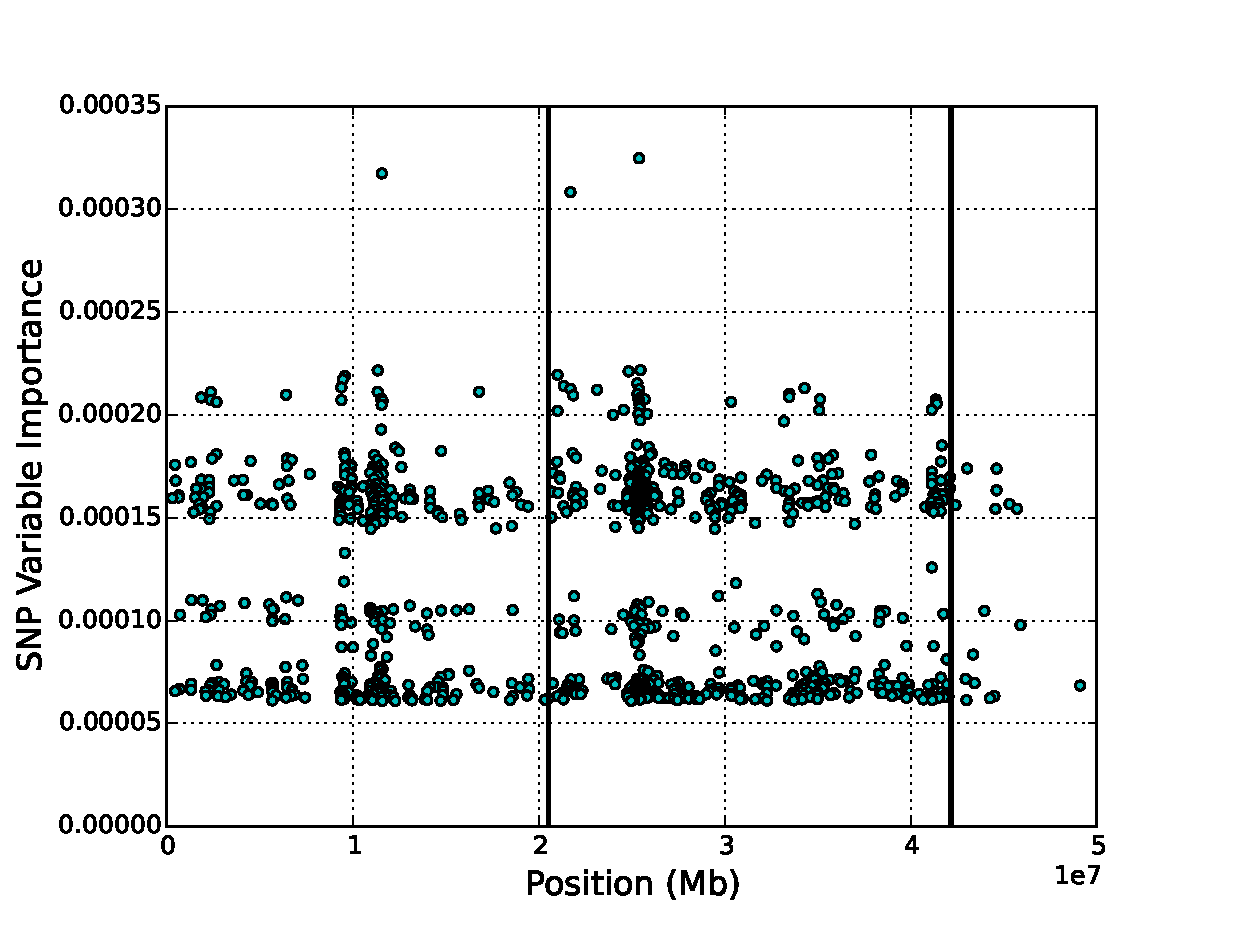
\includegraphics[width=\textwidth]{figures/random_forests/anopheles_2L_importances}
    \caption{Chromosome 2L}
    \label{fig:anopheles-2l}
  \end{subfigure}
  ~
  \begin{subfigure}[b]{0.45\textwidth}
    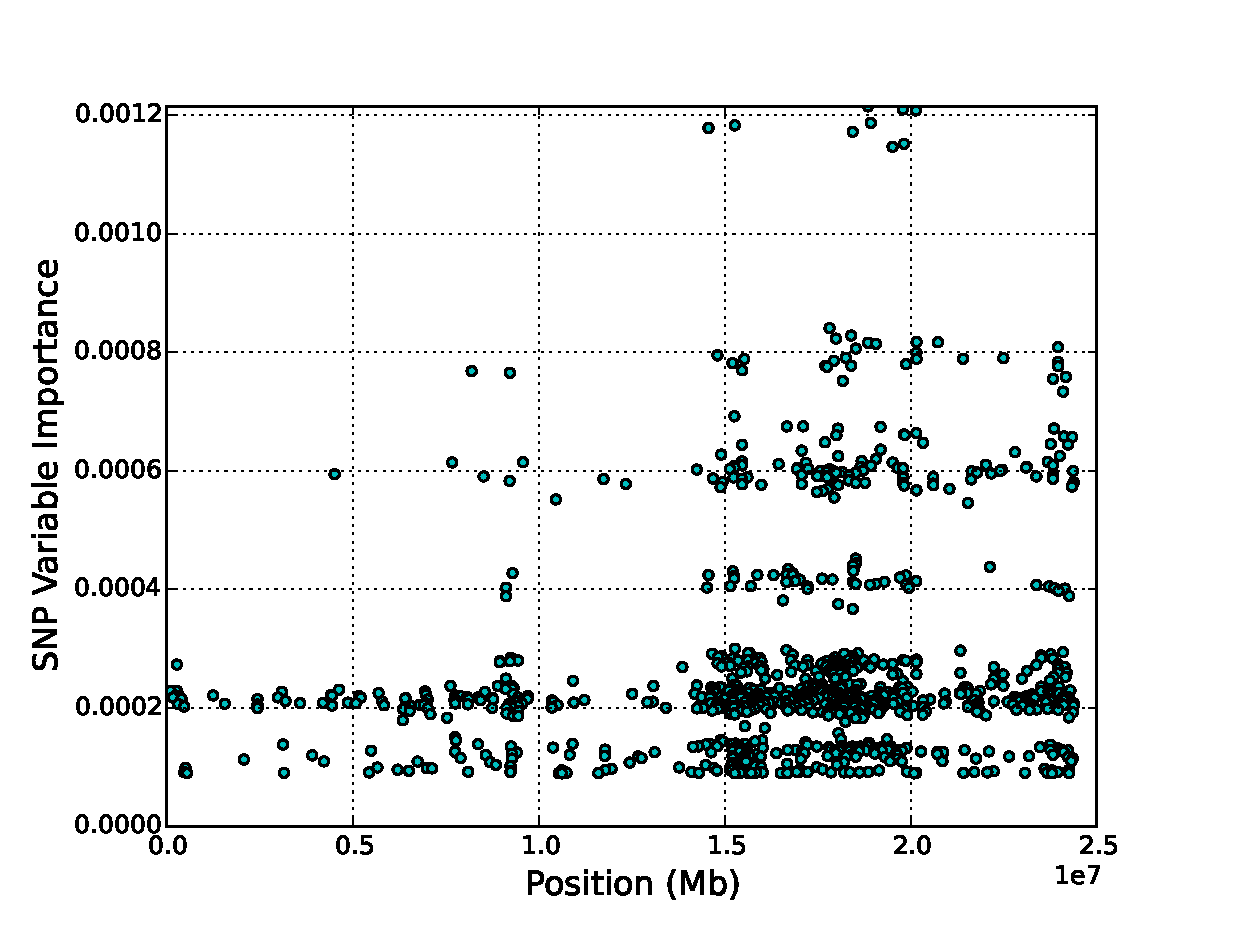
\includegraphics[width=\textwidth]{figures/random_forests/anopheles_X_importances}
    \caption{Chromosome X}
    \label{fig:anopheles-x}
  \end{subfigure}
  \caption{SNP Variable Importances for 2L and X chromosomes of \emph{An. gambiae} vs \emph{An. colluzzi}.  The cyan circles indicate the SNP variable importances.  The black lines bound the 2La inversion.}
  \label{fig:ranking-convergence-analysis}
\end{figure}

\begin{figure}[H]
  \centering
  \begin{subfigure}[b]{0.45\textwidth}
    \includegraphics[width=\textwidth]{figures/random_forests/funestus_ranks_10resamples_1000000trees_scores}
    \caption{All SNPs}
    \label{fig:funestus-all}
  \end{subfigure}
  ~
  \begin{subfigure}[b]{0.45\textwidth}
    \includegraphics[width=\textwidth]{figures/random_forests/funestus_ranks_10resamples_1000000trees_scores_subset}
    \caption{VIMs $> 10^{-4}$}
    \label{fig:funestus-thresholded}
  \end{subfigure}
  \caption{Variable importance scores of \emph{An. funestus} SNPs.}
  \label{fig:funestus}
\end{figure}
